\documentclass[draft]{article}
\usepackage[T2A]{fontenc}
\usepackage[utf8]{inputenc}
\usepackage[russian]{babel}
\usepackage{enumerate}
\usepackage{layout}
\usepackage{amsmath}
\usepackage{amssymb}
\usepackage[pdftex]{graphicx}
\usepackage{gensymb}
\usepackage{multirow}
\usepackage{python}
\usepackage[12pt]{extsizes}
\usepackage{hyperref}
\usepackage{xcolor}

\definecolor{linkcolor}{HTML}{3641fb} % цвет ссылок
\definecolor{urlcolor}{HTML}{799B03} % цвет гиперссылок
 
\hypersetup{pdfstartview=FitH,  linkcolor=linkcolor,urlcolor=urlcolor, colorlinks=true}

\textwidth = 16.5cm 
\textheight = 23cm 
\oddsidemargin = 0cm 
\topmargin = -2cm 
\headheight = 0mm 
\marginparwidth = 25mm 
\headsep = 0mm 
\baselineskip = 2mm 

\DeclareMathSizes{12}{13}{10}{10}

\title{Краткий сборник МФПЭ}
\author{571}

\begin{document}
\maketitle
\setcounter{secnumdepth}{-1}
\tableofcontents

\section{Предисловие}
Сборник всея знаний, кои должны были мы принять и усвоить за прошедшие годы в университете и не только.\\\\
Правила:
\begin{enumerate}
    \item Вода --- плохо
    \item Закапываться в дебри --- тоже плохо
    \item Краткость --- сестра таланта
\end{enumerate}

\section{Математика}




\subsection{Математический анализ}
\subsubsection{Точки разрыва аналитической функции}
\begin{enumerate}
    \item ТР первого рода
Точка разрыва первого рода при $x=a$, если:
\begin{itemize}
    \item Существуют левосторонний $\lim\limits_{x\to a-0}$ и правосторонний $\lim\limits_{x\to a+0}$ пределы;
    \item Эти пределы конечны.
\end{itemize}
Различают два вида точек разрыва первого рода:
\begin{itemize}
    \item Точка устранимого разрыва
    $$\lim\limits_{x\to a-0}f(x) = \lim\limits_{x\to a+0}f(x)$$
    \item Точка конечного разрыва
    $$\lim\limits_{x\to a-0}f(x)\neq \lim\limits_{x\to a+0}f(x)$$
\end{itemize}
Скачок функции:
$$\left|\lim\limits_{x\to a-0}f(x) - \lim\limits_{x\to a+0}f(x)\right|$$
\item ТР второго рода
Точка разрыва второго рода при $x=a$, если по крайней мере один из односторонних пределов не существует или равен бесконечности.
\end{enumerate}

\subsubsection{Системы координат}
\begin{enumerate}
    \item Декартова СК
    \item Цилиндрическая СК\\
      Связь с декартовыми координатами
      \begin{equation*}
        \begin{cases}
          $$x=rcos\phi$$\\
          $$y=rsin\phi$$\\
          $$z=z$$
        \end{cases}
      \end{equation*}
      Якобиан: $$J=r$$
\end{enumerate}



\subsection{Ряд Фурье}
\subsubsection{Условия Дирихле}
Для того чтобы было возможно разложить функцию в ряд Фурье должны выполнятся \textbf{условия Дирихле}:
\begin{enumerate}
    \item Влюбом конечном интервале функция колебания s(t) должна быть непрерывна или иметь конечное число разрывов первого рода;
    \item В пределах одного периода функция s(t) должна иметь конечное число максимумов и минимумов.
\end{enumerate}

\subsubsection{Аналитическая форма}
$$s(t)\approx\frac{a_{0}}{2}+\sum\limits_{n=1}^{\infty}\left(a_{n}cos\left(\frac{2\pi n}{T}t\right)+b_{n}sin\left(\frac{2\pi n}{T}t\right)\right)$$

$$a_{0}=\frac{2}{T}\int\limits_{0}^{T}s(t)dt$$
$$a_{n}=\frac{2}{T}\int\limits_{0}^{T}s(t)cos\left(\frac{2\pi n}{T}t\right)dt$$
$$b_{n}=\frac{2}{T}\int\limits_{0}^{T}s(t)sin\left(\frac{2\pi n}{T}t\right)dt$$

Или:
$$s(t)\approx\frac{a_{0}}{2}+\sum\limits_{n=1}^{\infty}A_{n}cos(\frac{2\pi n}{T}t-\phi_{n})$$
$$A_{n}=\sqrt{a_{n}^{2}+b_{n}^{2}}$$
$$\phi_{n}=arctg\left(\frac{b_{n}}{a_{n}}\right)$$

\noindent$A_{n}$ --- \textbf{Амплитудный спектр}\\
$\phi_{n}$ --- \textbf{Фазовый спектр}

\subsubsection{Комплексная форма}

$$cos\left(\frac{2\pi n}{T}t-\phi_{n}\right)=\frac{1}{2}(e^{i\left(\frac{2\pi n}{T}t-\phi_{n}\right)}+e^{-i\left(\frac{2\pi n}{T}t-\phi_{n}\right)})$$

Тогда:
$$s(t)=\frac{1}{2}\sum\limits_{n=-\infty}^{n=\infty}C_{n}e^{i\frac{2\pi n}{T}t}$$
$$C_{n}=\frac{2}{T}\int\limits_{0}^{T}s(t)e^{-i\frac{2\pi n}{T}t}dt$$
$C_{0}=a_{0}$\\
$C_{n}=A_{n}e^{-i\phi_{n}}$\\
$C_{-n}=A_{n}e^{i\phi_{n}}$\\
$|C_{n}|=|C_{-n}|=A_{n}$
\\\\
Комплексные амплитуды $C_{n}$ и $C_{-n}$ являются взаимно сопряженными комплексными величинами:$$C_{-n}=C_{n}^{*}$$

\subsubsection{Интеграл Фурье}
Используется для разложения непереодических сигналов.\\
Спектр непереодических сигналов в отличии от переодических является сплошным.\\
Подставим $C_{n}=\frac{2}{T}\int\limits_{t_{1}}^{t_{2}}s(t)e^{-i\frac{2\pi n}{T}t}dt$ в $s(t)=\frac{1}{2}\sum\limits_{n=-\infty}^{n=\infty}C_{n}e^{i\frac{2\pi n}{T}t}$, получим:
$$s(t)=\sum\limits_{n=-\infty}^{n=\infty}\frac{1}{T}\left[\int\limits_{t_{1}}^{t_{2}}s(t)e^{-i\frac{2\pi n}{T}t}dt\right]e^{i\frac{2\pi n}{T}t}$$
$$\frac{1}{T}=\frac{\omega_{0}}{2\pi}$$
$$s(t)=\frac{1}{2\pi}\sum\limits_{n=-\infty}^{n=\infty}\left[\int\limits_{t_{1}}^{t_{2}}s(t)e^{-i\frac{2\pi n}{T}t}dt\right]e^{i\frac{2\pi n}{T}t}\omega_{0}$$

При $T\longrightarrow\infty$: $\omega_{0}\longrightarrow d\omega$, $n\omega_{0}\longrightarrow \omega$, $\sum\longrightarrow\int$

$$s(t)=\frac{1}{2\pi}\int\limits_{-\infty}^{\infty}e^{i\omega t}\int\limits_{t_{1}}^{t_{2}}s(t)e^{-i\omega t}dt$$
$$S(\omega)=\int\limits_{t_{1}}^{t_{2}}s(t)e^{-i\omega t}dt$$
$$s(t)=\frac{1}{2\pi}\int\limits_{-\infty}^{\infty}S(\omega)e^{i\omega t}dt$$
Данное выражение позволяет представить непереодическую функцию в виде суммы гармонических колебаний с бесконечно малыми гармониками.\\

\subsubsection{Разложение неинтегрируемых функций}

\subsubsection{Дискретное преобразование Фурье}

\subsection{Вариационное исчисление}

\subsubsection{Введение}
Задача - найти вид функции $f(r_{1},...,r_{n})$
$$\mathcal{V}[f(r_{1},...,r_{n})]$$
$\mathcal{V}$ - Функционал\\
$$\mathcal{V} - \text{экстремален}\longrightarrow\delta\mathcal{V}=0$$
Как считать вариацию($\delta\mathcal{V}$):
$$\delta\mathcal{V}=\left(\frac{\partial}{\partial\alpha}\mathcal{V}[y+\alpha\delta y]\right)_{\alpha=0}$$

\subsubsection{Уравнение Эйлера}
Задача:
\begin{equation*}
 \begin{cases}
   $$\mathcal{V}[y(x)]=\int_{a}^{b}\mathcal{F}(x,y(x),y'(x))dx$$\\
   $$\text{Граничное условие:} y(a)=A;y(b)=B$$\\
   $$y(x)-?: \mathcal{V} - \text{экстремален}$$
 \end{cases}
\end{equation*}\\
Способ найти решение - Уравнение Эйлера:
$$\frac{\partial \mathcal{F}}{\partial y}-\frac{d}{dx}\frac{\partial \mathcal{F}}{\partial y'}=0$$
Частные учаи:
\begin{enumerate}
    \item $\mathcal{F}=\mathcal{F}(x,y'(x))$
    $$\frac{\partial \mathcal{F}}{\partial y'}=c$$
    \item $\mathcal{F}=\mathcal{F}(y(x),y'(x))$
    $$\mathcal{F}-y'\frac{\partial \mathcal{F}}{\partial y'}=c$$
\end{enumerate}

\subsubsection{Система уравнений Эйлера}
$y_{i}$ можно варьировать по очереди\\
Задача:
\begin{equation*}
 \begin{cases}
   $$\mathcal{V}[y_{1},...,y_{n}]=\int_{a}^{b}\mathcal{F}(x,y_{1}(x),...y_{n}(x),y_{1}'(x),...y_{n}'(x))dx$$\\
   $$\text{Граничное условие:} y_{i}(a)=A_{i};y_{i}(b)=B_{i}$$\\
   $$y_{i}(x)-?: \mathcal{V} - \text{экстремален},i=1,2,...,n$$
 \end{cases}
\end{equation*}\\
Решение - система уравнений Эйлера:
$$\frac{\partial \mathcal{F}}{\partial y_{i}}-\frac{d}{dx}\frac{\partial \mathcal{F}}{\partial y_{i}'}=0$$

\subsubsection{Вариационные задачи с дифференциальной связью}
На искомую функцию накладывается ограничение дифференциального вида
\begin{equation*}
 \begin{cases}
   $$\mathcal{V}[y_{1},...,y_{n}]=\int_{a}^{b}\mathcal{F}(x,y_{1}(x),...y_{n}(x),y_{1}'(x),...y_{n}'(x))dx$$\\
   $$G(x,y_{1}(x),...y_{n}(x),y_{1}'(x),...y_{n}'(x))=0-\text{Связь}$$\\
   $$\text{Граничное условие:} y_{i}(a)=A_{i};y_{i}(b)=B_{i}$$\\
   $$y_{i}(x)-?: \mathcal{V} - \text{экстремален},i=1,2,...,n$$
 \end{cases}
\end{equation*}\\
В данном случае Функционал $\mathcal{F}$ принимает вид:
$$\mathcal{F}^{*}=\mathcal{F}+\lambda (x) G$$
где $\lambda (x)$ - множитель Лагранжа\\\\
И система уравнений Эйлера сводится к виду:
\begin{equation*}
 \begin{cases}
   $$\frac{\partial \mathcal{F}^{*}}{\partial y_{i}}-\frac{d}{dx}\frac{\partial \mathcal{F}^{*}}{\partial y_{i}'}=0; i=1,n$$\\
   $$G(x,y_{1}(x),...y_{n}(x),y_{1}'(x),...y_{n}'(x))=0$$
 \end{cases}
\end{equation*}\\

\subsubsection{Вариационные задачи с интегральной связью (изопериметрические задачи)}
Постановка задачи:
\begin{equation*}
 \begin{cases}
   $$\mathcal{V}[y_{1},...,y_{n}]=\int_{a}^{b}\mathcal{F}(x,y_{1}(x),...y_{n}(x),y_{1}'(x),...y_{n}'(x))dx$$\\
   $$\int\limits_{a}^{b}G(x,y_{1}(x),...y_{n}(x),y_{1}'(x),...y_{n}'(x))=c\;\;(c - \text{известная const})$$\\
   $$\text{Граничное условие:} y_{i}(a)=A_{i};y_{i}(b)=B_{i}$$\\
   $$y_{i}(x)-?: \mathcal{V} - \text{экстремален},i=1,2,...,n$$
 \end{cases}
\end{equation*}\\
Алгоритм решения изопериметрических задач:
\begin{enumerate}
    \item Ввести $\mathcal{F}^{*}=\mathcal{F}+\lambda G$\\ В данном случае $\lambda=const$
    \item Решить УЭ для $\mathcal{F}$\\ Решение будет содержать $n$ констант $c_{i}$ и $\lambda$
    \item Получившиеся неизвестные константы находим используя граничные условия и условие связи:\\
    $\int\limits_{a}^{b}G(x,y_{1}(x),...y_{n}(x),y_{1}'(x),...y_{n}'(x))=c$
\end{enumerate}

\subsubsection{Уравнение Эйлера-Остроградского}
Уравнение для n-мерного функционала.\\
Пример с функционалом одной n-мерной функции:
\begin{equation*}
 \begin{cases}
   $$\mathcal{V}[f(x_{1},...,x_{n})]=\int...\int\mathcal{F}(x_{1},...,x_{n},f(x_{1},...,x_{n}),f^{'}_{x_{1}},...,f^{'}_{x_{n}})dx$$\\
   $$\text{Граничное условие:} f|_{\sigma}=\phi(x_{1},...,x_{n})-\text{известная ф-ия}\longrightarrow\delta f|_{\sigma}=0$$\\
   $$f - ?: \mathcal{V} - \text{экстремален}$$
 \end{cases}
\end{equation*}\\
Уравнение Эйлера:
$$\frac{\partial \mathcal{F}}{\partial f}-\sum_{i=1}^{n}\frac{d}{dx_{i}}\frac{\partial \mathcal{F}}{\partial f'_{x_{i}}}=0$$

\subsubsection{Задачи с подвижными границами}

\begin{figure}[h!]
\begin{center}
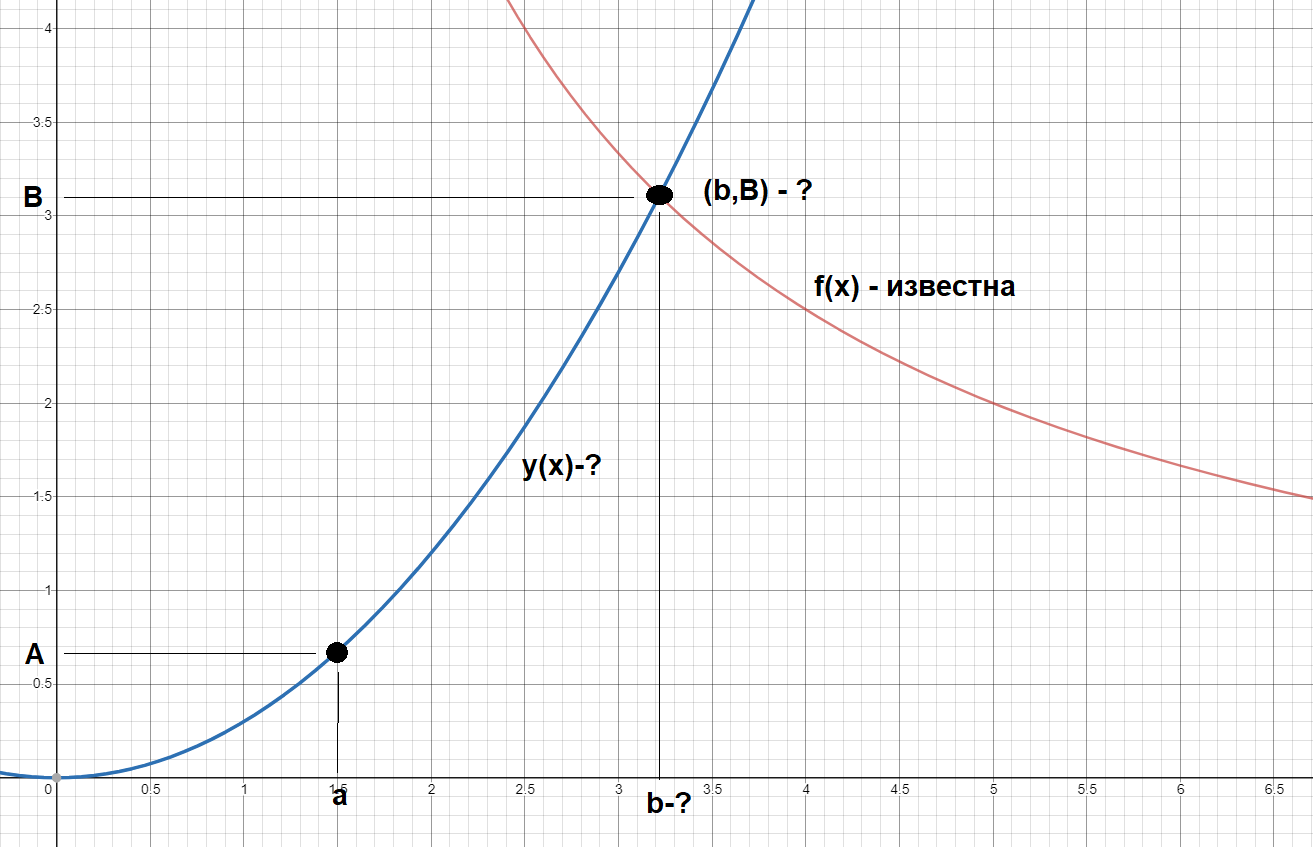
\includegraphics[width = 12.5cm]{Math/variable_border_example.png}
\end{center}
\end{figure}

Общий случай:
\begin{equation*}
 \begin{cases}
   $$\mathcal{V}[y(x)]=\int\limits_{a}^{b}\mathcal{F}(x,y,y')dx$$\\
   $$y(a)=A-\text{a и A известны}$$\\
   $$y(b)=B=f(b)-\text{b-известно,$f(b)$-неизвестно}$$\\
   $$y(x) - ?: \mathcal{V} - \text{экстремален}$$
 \end{cases}
\end{equation*}
Логика решения:
\begin{itemize}
    \item Этап 1\\
    Фиксируем $B$, решаем вариационную задачу и получаем решение
    $$y=y(x,B)$$
    \item
    Освобождаем координату $B$
    $$\frac{\partial\mathcal{V}}{\partial B}=0$$
\end{itemize}
Решение общего случая:
\begin{itemize}
    \item Сначала решаем вариационную задачу с неизвестным $B$ и получаем решение
    $$y=y(x,B)$$
    \item Второй этап --- применяем условие трансверсальности
    $$\left\{\mathcal{F}+[f'(x)-y'(x)]\frac{\partial \mathcal{F}}{\partial y'}\right\}_{x=b}=0$$
\end{itemize}

Частные случаи:
\begin{enumerate}
    \item $$f'(x)= \infty$$
          \begin{figure}[h!]
            \begin{center}
              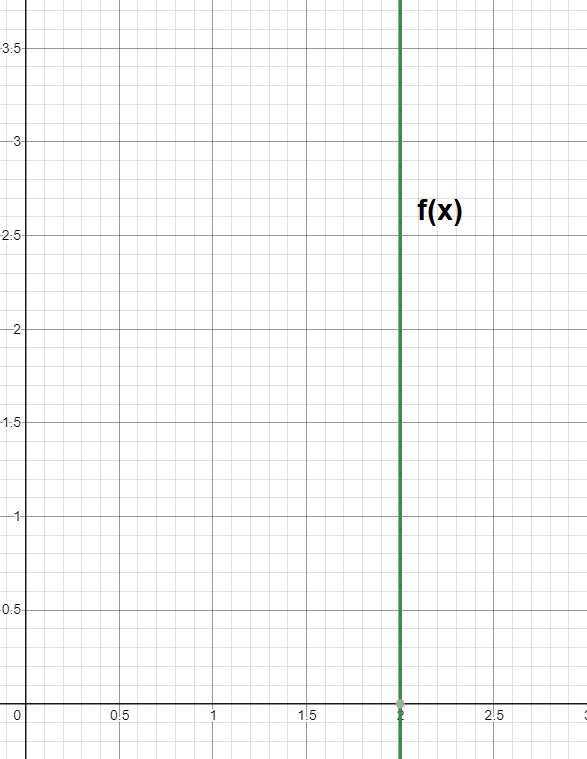
\includegraphics[width = 8cm]{Math/infty_border_func.png}
            \end{center}
          \end{figure}
          \\
          Условие трансверсальности:
          $$\left\{\frac{\partial\mathcal{F}}{\partial y'}\right\}_{x=B}=0$$
    \item 
      \begin{equation*}
        \begin{cases}
          $$\mathcal{V}[y(x)]=\int\limits_{a}^{b}\mathcal{F}(x,y,y')dx$$\\
          $$y(a)=A$$\\
          $$y(b)=B$$
        \end{cases}
      \end{equation*}
      
      \begin{figure}[h!]
        \begin{center}
          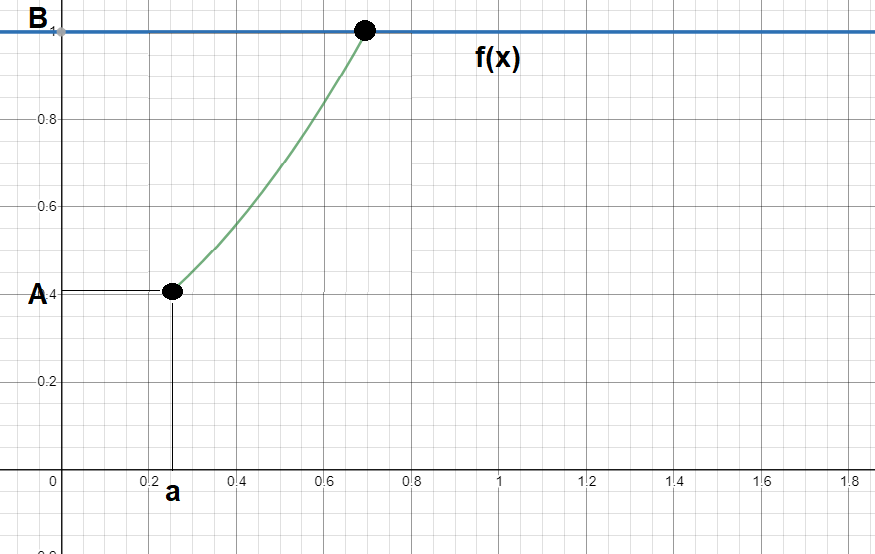
\includegraphics[width = 10cm]{Math/option_b.png}
        \end{center}
      \end{figure}
      
      Условие трансверсальности:
      $$\left\{\mathcal{F}-y'\frac{\partial\mathcal{F}}{\partial y'}\right\}_{x=B}=0$$
      
    \item Свободный конец\\
    
    \begin{figure}[h!]
        \begin{center}
          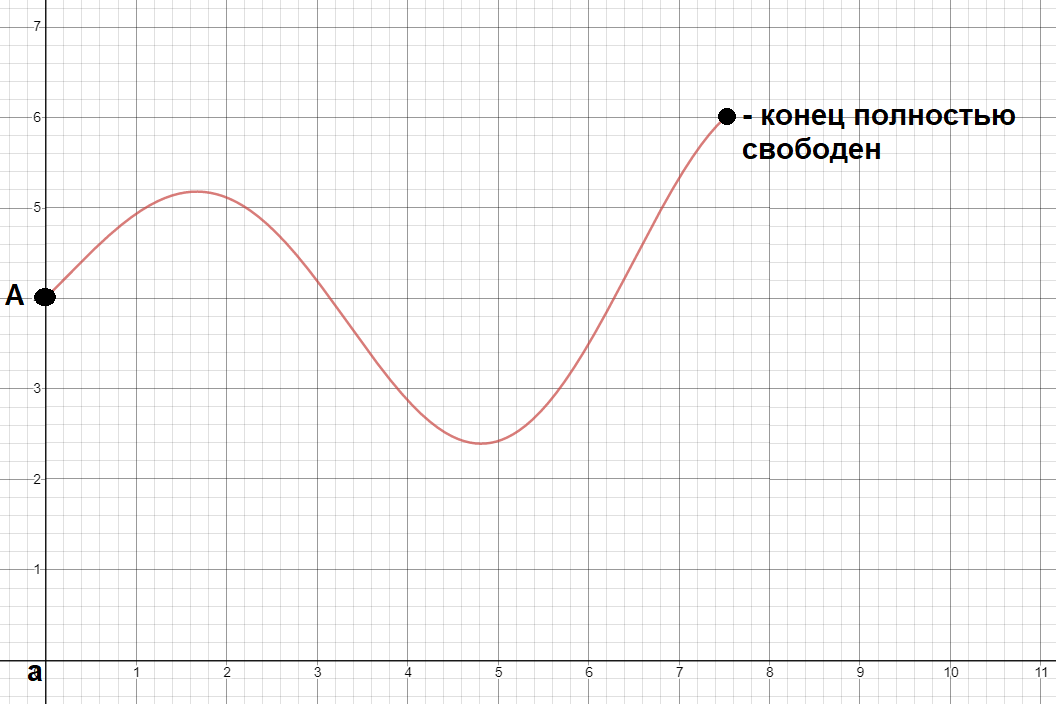
\includegraphics[width = 10cm]{Math/h.png}
        \end{center}
    \end{figure}
    
    Освобождаем координаты $B$ и $b$ по очереди и получаем систему уравнений трансверсальности
    \begin{equation*}
        \begin{cases}
          $$\left\{\frac{\partial\mathcal{F}}{\partial y'}\right\}_{x=B}=0$$\\
          $$\left\{\mathcal{F}-y'\frac{\partial\mathcal{F}}{\partial y'}\right\}_{x=B}=0$$
        \end{cases}
      \end{equation*}
\end{enumerate}




\subsection{Интегральные уравнения}
\subsubsection{Основные типы линейных ИУ}
$f(x)-\text{свободный член}$\\
$K(x,S)-\text{ядро}$\\
$y$ - искомая функция
\begin{enumerate}
    \item Уравнения Фредгольма
    \begin{enumerate}
        \item 1-го рода
        $$f(x)=\int\limits_{a}^{b}K(x,S)y(S)dS$$
        \item 2-го рода
        \begin{itemize}
            \item Однородное:
            $$y(x)=\lambda\int\limits_{a}^{b}K(x,S)y(S)dS$$
            \item Неоднородное:
            $$y(x)=f(x)+\lambda\int\limits_{a}^{b}K(x,S)y(S)dS$$
        \end{itemize}
    \end{enumerate}
    \item Уравнения Вальтерры
    \begin{enumerate}
        \item 1-го рода
        $$y(x)=\int\limits_{a}^{x}K(x,S)y(S)dS$$
        \item 2-го рода
        $$y(x)=f(x)+\lambda\int\limits_{a}^{x}K(x,S)y(S)dS$$
    \end{enumerate}
\end{enumerate}

\subsubsection{Уравнение Фредгольма второго рода с вырожденным ядром}
$$y(x)=f(x)+\lambda\int\limits_{a}^{b}K(x,S)y(S)dS$$
Вырожденные и невырожденные ядра
\begin{itemize}
  \item Вырожденные: $$K(x,S)=\sum\limits_{j=1}^{n<\infty}\alpha_{j}(x)\beta_{j}(S)$$
     Примеры: $K(x,S)=1,x,S,xS,x+S,e^{x+S},sin(x+S),...$
  \item Невырожденные: $K(x,S)=e^{xS},sin(xS),\sqrt{x+S}$
  \\\\
  Метод решения:
  \begin{enumerate}
      \item $$y(x)=f(x)+\lambda\sum\limits_{j=1}^{n<\infty}\alpha_{j}(x)\int\limits_{a}^{b}\beta_{j}(S)y(S)dS$$
      $$\int\limits_{a}^{b}\beta_{j}(S)y(S)dS=const=\tilde y_{j}$$
      $$y(x)=f(x)+\lambda\sum\limits_{j=1}^{n<\infty}\alpha_{j}(x)\tilde y_{j}\;\;\;\;(1)$$
      \item Домножаем левую и правую части уравнения (1) на $\beta_{i}(x),i\in [1,n]$\\
      Затем интегрируем по $x$ от $a$ до $b$: $\int\limits_{a}^{b}dx$\\
      Получаем:
      $$\int\limits_{a}^{b}\beta_{i}(x)y(x)dx=\tilde y_{i}$$
      $$\int\limits_{a}^{b}\beta_{i}(x)f(x)dx=\tilde f_{i}$$
      $$\int\limits_{a}^{b}\beta_{i}(x)\alpha_{j}(x)dx=K_{ij}$$
      $$\tilde y_{j}=\tilde f_{i} + \lambda\sum\limits_{j=1}^{n}K_{ij}\tilde y_{j}$$
  \end{enumerate}
  


\subsection{Дискретная математика}
\subsubsection{Скобка Айверсона}
\begin{equation*}
[P] = 
 \begin{cases}
   1, &\text{если $P$ истинно}\\
   0, &\text{если $P$ ложно}
 \end{cases}
\end{equation*}
Пример (Частный случай --- символ Кронекера):
$$\delta_{ij}=[i=j]$$
\end{itemize}
\clearpage
\section{Физика}
\subsection{Механика}
\subsubsection{Уравнение Эйлера-Лагранжа}
Лагранжиан:
$$L(q_{i},\dot q_{i},t)=T-V$$
$T$ - кинетическая энергия системы\\
$V$ - потенциальная энергия системы\\
n - число степеней свободы\\\\
Уравнение Эйлера-Лагранжа для $n$ степеней совободы:
\begin{equation*}
 \begin{cases}
   $$\frac{d}{dt}\frac{\partial L}{\partial \dot q_{1}}-\frac{\partial L}{\partial q_{1}} = 0$$\\
   $$\frac{d}{dt}\frac{\partial L}{\partial \dot q_{2}}-\frac{\partial L}{\partial q_{2}} = 0$$\\
   ...\\
   $$\frac{d}{dt}\frac{\partial L}{\partial \dot q_{n}}-\frac{\partial L}{\partial q_{n}} = 0$$
 \end{cases}
\end{equation*}

\subsubsection{Интегралы движения}
Уравнение движения имеет вид:
$$\ddot q = F(q,\dot q,t)$$
Для $n$ степеней свободы:
$$q = q(q_{1},...,q_{n})$$
$q$ - обобщенный вектор координат
\begin{equation*}
 \begin{cases}
   $$\ddot q_{1} = F(q_{1},...,q_{n},\dot q_{1},...,\dot q_{n},t)$$\\
   $$\ddot q_{2} = F(q_{1},...,q_{n},\dot q_{1},...,\dot q_{n},t)$$\\
   ...\\
   $$\ddot q_{n} = F(q_{1},...,q_{n},\dot q_{1},...,\dot q_{n},t)$$
 \end{cases}
\end{equation*}
При решении данной системы дифференциальных уравнений второго порядка получим решение:
$$q=q(t,C_{1},C_{2},...,C_{2n})$$
$C_{1},C_{2},...,C_{2n}$ - константы, называемые интегралами движения.\\\\
Три "главных" интеграла движения:
\begin{enumerate}
    \item Время однородно - уравнение движения системы не зависит от начального момента времени
    $$L=L(q,\dot q)\longrightarrow \frac{dL}{dt}=0$$
    $$\sum_{i}\frac{\partial L}{\partial \dot q_{i}}\dot q-L=const=E$$
    Полная энергия замкнутой системы не меняется;
    \item Пространство однородно - уравнение движения системы сохраняется при смещении ее в пространстве (При отсутствии влияния внешних полей и объектов)
    $$L=L(t,q)$$
    $$\sum_{i}\frac{\partial L}{\partial \dot q_{i}}=const=\textbf{P}$$
    Закон сохранения импульса;
    \item Пространство изотропно - при повороте системы вокруг некой оси уравнение движения не меняется.\\
    $\overline{\varphi}$ - вектор угла поворота системы (перпендикулярен плоскости вращения, по модулю равен углу поворота)\\
    Изменения обобщенных координат и скорости выражаются через векторные произведения:
    \begin{equation*}
     \begin{cases}
       $$\delta q=[\delta\overline{\varphi},q]$$\\
       $$\delta\dot q=[\delta\overline{\varphi},\dot q]$$
     \end{cases}
    \end{equation*}
    $$\delta L = \sum_{i} \frac{\partial L}{\partial q_{i}}\delta q_{i} + \frac{\partial L}{\partial \dot q_{i}}\delta \dot q_{i} =\left\{\frac{\partial L}{\partial q_{i}} = \dot p_{i}, \frac{\partial L}{\partial \dot q_{i}} = p_{i} \right\}= \delta \overline{\varphi}\frac{d}{dt}\sum_{i}\textbf{q}_{i}\times \textbf{p}_{i}=0$$
    $$\sum_{i}\textbf{q}_{i}\times \textbf{p}_{i} = const = \textbf{L}$$
    Закон сохранения момента импульса
\end{enumerate}


\subsection{Общая теория колебаний}
\clearpage
%\begin{document}

\section{Программирование}


\subsection{Численные методы}

\subsubsection{Аппроксимация}
Известны данные $(t_{i},b_{i});i=1,...,m$
$$b(t)-?$$
Рассмотрим линейную модель (комбинация модельных функций линейна)
$$b_{i}=x_{1}\phi_{1}(t_{i})+x_{2}\phi_{2}(t_{i})+...+x_{n}\phi_{n}(t_{i})$$
$\phi_{i}(t)-$модельные функции(задаем сами)\\
$x_{i}-$параметры модели\\\\
Введем матрицу $A$ $m\times n$, где $m$-число данных, $n$-количество модельных функций
$$a_{ij}=\left(A\right)_{ij}=\phi_{j}(t_{i})$$
\begin{equation*}
A = \left(
\begin{array}{cccc}
\phi_{1}(t_{1}) & \phi_{2}(t_{1}) & \ldots & \phi_{n}(t_{1})\\
\phi_{1}(t_{2}) & \phi_{2}(t_{2}) & \ldots & \phi_{n}(t_{2})\\
\vdots & \vdots & \ddots & \vdots\\
\phi_{1}(t_{m}) & \phi_{2}(t_{m}) & \ldots & \phi_{n}(t_{m})
\end{array}
\right)
\end{equation*}
В таком случае задачу можно переписать в виде:
$$b\approx Ax\Longrightarrow b-Ax\approx 0$$
$r=b-Ax$ --- вектор невязок\\
$$r\longrightarrow 0\Leftrightarrow \min_{x}\sum_{j=1}^{m}[(b-Ax)_{j}]^{2}=\min_{x}||b-Ax||_{2}^{2}=(b-Ax)^{T}(b-Ax)$$
Можно ввести веса $\omega_{j}:$ $$\min_{x}\sum_{j=1}^{m}[\omega_{j}(b-Ax)_{j}]^{2}$$
где $\omega_{j}=\frac{1}{\epsilon_{j}}$,$\epsilon_{j}$ --- ошибка измерения в $j$-ой точке\\\\
\textbf{Нахождение параметров модели:}
\begin{enumerate}
    \item Нормальные уравнения
    $$r^{2}=(b-Ax)^{T}(b-Ax)=b^{T}b-2b^{T}Ax+x^{T}A^{T}Ax\longrightarrow min$$
    $$\frac{d(r^{2})}{dx}=0\Longrightarrow (A^{T}A)x=(A^{T}b)$$
    \item Ортоганальные факторизации\\
    Ортоганальное преобразование --- домножение на $P$: $P^{T}P=1$
    \item Преобразование Хаусхолдера
    $$P=1-2\frac{\mathcal{V}\mathcal{V}^{T}}{\mathcal{V}^{T}\mathcal{V}}$$
    Позволяет привести матрицу $A$ к верхнетреугольному виду, сохраняя норму.\\
    Пусть $a$ --- произвольный вектор-столбец, тогда:
    \begin{equation*}
    a = \left(
    \begin{array}{cccc}
    a_{1}\\
    a_{2}\\
    \vdots\\
    a_{m}
    \end{array}
    \right)
    \end{equation*}
    \begin{equation*}
    Pa = \left(
    \begin{array}{cccc}
    \alpha\\
    0\\
    \vdots\\
    0
    \end{array}
    \right)
    \end{equation*}
    $\alpha=||a||_{2}$\\\\
    Пример:
\begin{equation*}
A = \left(
\begin{array}{cccc}
\times & \times & \times \\
\times & \times & \times \\
\times & \times & \times \\
\times & \times & \times
\end{array}
\right)
\end{equation*}
\begin{equation*}
PA = \left(
\begin{array}{cccc}
\alpha & \times & \times \\
0 & \times & \times \\
0 & \times & \times \\
0 & \times & \times
\end{array}
\right)
\end{equation*}
\begin{equation*}
P_{1}PA = \left(
\begin{array}{cccc}
1 & 0 \\
0 & \overline{P}
\end{array}
\right)
\left(
\begin{array}{cccc}
\alpha & \times & \times \\
0 & \overline{\alpha} & \times \\
0 & 0 & \times \\
0 & 0 & \times
\end{array}
\right)
\end{equation*}
\begin{equation*}
P_{2}P_{1}PA = \left(
\begin{array}{cccc}
1 & 0 & 0\\
0 & 1 & 0\\
0 & 0 & \widetilde{P}
\end{array}
\right)
\left(
\begin{array}{cccc}
\alpha & \times & \times \\
0 & \overline{\alpha} & \times \\
0 & 0 & \widetilde{\alpha} \\
0 & 0 & 0
\end{array}
\right)
\end{equation*}
Формула для $\mathcal{V}$:\\
$$Pa=\alpha(1,0,...,0)^{T}=\alpha e_{1}\Longrightarrow Pa=\left(P=1-2\frac{\mathcal{V}\mathcal{V}^{T}}{\mathcal{V}^{T}\mathcal{V}}\right)a=\alpha e_{1}$$
Отсюда:
$$\mathcal{V}=a\pm ||a||_{2}e_{1}$$
    \end{enumerate}

%\end{document}
\clearpage
\section{Электроника}

\subsection{Полупроводниковая электроника}

\end{document}